\documentclass{article}
\usepackage{geometry}
\geometry{
letterpaper, portrait, margin=1in
}
\usepackage{multirow}
\usepackage{graphicx}
\graphicspath{{graphs/}}

\begin{document}

\title{Cmsc 191 Final Exam: Analyzing the Performances of the Genetic Algorithm (GA), Simulated Annealing (SA) and Hybrid Simulated Annealing (SAGA) on Five Test Functions.}

\author{Gimel David F. Velasco}

\date{December 13, 2016}

\maketitle

\abstract{This paper demonstrates an implementation of the Genetic Algorithm, Simulated Annealing and Hybrid Simulated Annealing in solving the global minimum for 5 continuous 5-variabled standard test functions. The performances based on time efficiency and solution accuracy of the three algorithms is then compared based on the tests that were conducted.}

\section{Introduction}
The \textbf{Genetic Algorithm (GA)} is an algorithm made by Holland on 1975. The Algorithm is inspired by the concept of Genetics and Natural Selection. It approaches a particular problem by looking for the fittest individual and considers it as the solution to the problem. It approaches a particular problem by looking for the fittest individual and considers it as the solution to the problem.\\

The \textbf{Simulated Annealing (SA)} is another type of Heuristics which is used for solving complex problems. This algorithm is of the analogy that if a liquid material cools slowly, the system will then get into a state of minimum energy optimally. On the onther hand, if the liquid material cools too quickly, it will have a sub-optimal configuration. Also, For these standard test functions, the Genetic Algorithm and Simulated Annealing Algorithm will solve or get close to their respective global minimum.\\

The \textbf{Hybrid Simulated Annealing (SAGA)} is the combination of both GA and SA wherein instead of looking at a single $X_i$ as the possible solution for a problem, a whole number of population of $X_i$s are used. Which was adapted in the concept of the Genetic Algorithm. Now, for these standard test functions, the Hybrid Simulated Annealing Algorithm will solve or get close to their respective global minimum.\\

\section{5 Test Functions}
The algorithm will seek the global minimum of the following standard test functions [1]:\\
\textbf{Problem 1}: De Jong's Function ($|x| \leq 5.12; n=5,10$)
\begin{equation}
f(x) = \sum^n_{i=1}x_i^2
\end{equation}
\centerline{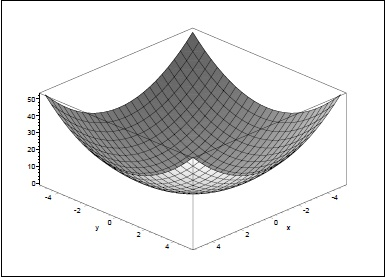
\includegraphics{tf1}}
Global Minimum: $f(x) = 0$\\\\
\textbf{Problem 2}: Axis Parallel Hyper-Ellipsoid Function ($|x| \leq 5.12; n=5,10$)
\begin{equation}
f(x) = \sum^n_{i=1}(i*x_i^2)
\end{equation}
\centerline{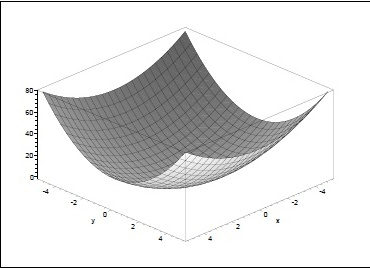
\includegraphics{tf2}}
Global Minimum: $f(x) = 0$\\\\
\textbf{Problem 3}: Rotated Hyper-Ellipsoid Function ($|x| \leq 65.536; n=5,10$)
\begin{equation}
f(x) = \sum^n_{i=1}\sum^i_{j=1}x_j^2
\end{equation}
\centerline{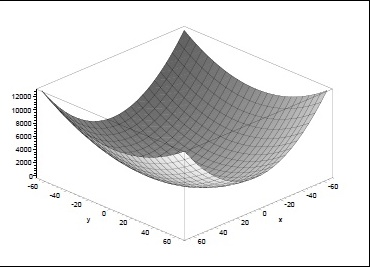
\includegraphics{tf3}}
Global Minimum: $f(x) = 0$\\\\
\textbf{Problem 4}: Rastrigin's Function ($|x| \leq 5.12; n=5,10$)
\begin{equation}
f(x) = 10n + \sum^n_{i=1}[x_i^2 - 10cos(2\pi x_i)]
\end{equation}
\centerline{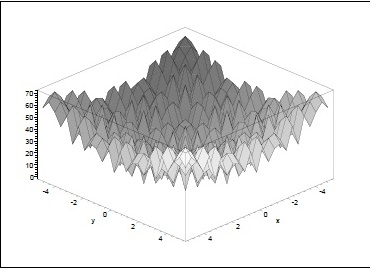
\includegraphics{tf4}}
Global Minimum: $f(x) = 0$\\\\
\textbf{Problem 5}: Ackley's Function ($|x| \leq 32.768; n=5,10$)
\begin{equation}
f(x) = -a*exp(-b*\sqrt{\frac{1}{n}\sum^n_{i=1}x_i^2}) - exp(\frac{1}{n}\sum^n_{i=1}cos(cx_i)) + a + exp(1)
\end{equation}
\centerline{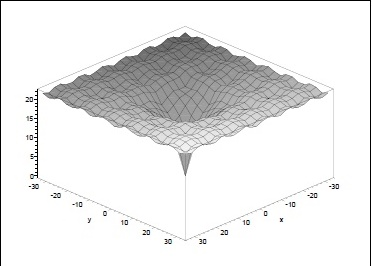
\includegraphics{tf6}}
Global Minimum: $f(x) = 0$\\
where $a=20, b=0.2, c = 2\pi$\\\\

\section{Methodology}
The fitness function or objective function of which is defined as:
\begin{equation}
OBJ(x) = |f(x) - global minimum|
\end{equation}

A Minimization Problem is implemented in the algorithm wherein the objective of the algorithm is to get very close if not equal to zero.

\subsection{The Genetic Algorithm}
The Genetic Algorithm implemented in this program is inspired by how the Genetic Algorithm is implemented in Hermawanto's article on solving a 4-tuple function. The pseudocode of the Genetic Algorithm implemented in the program is shown below:\\
\textit{
1. Determine the number of chromosomes, population, generation, mutation rate and crossover rate value\\
2. Generate first generation of chromosomes\\
3. Tournament Selection of the quarter of the population\\
3. Crossover of the selected parents based on the crossover rate\\
4. Mutation of part of the generation according to the mutation rate\\
6. Evaluation of fitness value of chromosomes by using the fitness function\\
7. Repeat steps 2-6 until the maximum number of generations is met or until desired fitness is reached\\
8. Solution (Best Chromosome)\\
}

A modification in the code was made. The algorithm tends stick to the fittest chromosome and mutates less randomly when the chromosomes get fitter and fitter. This is done so that the algorithm would be able to be much more exact and precise in looking for the global minimum.

\subsection{The Simulated Annealing Algorithm}
The Simulated Annealing Algorithm implemented in this program is based on how the algorithm is explained in the presentation made by Oliver de Weck, Ph.D. The pseudocode of the Simulated Annealing Algorithm is shown below:\\
\textit{
1. Choose a random Xi, select the initial system temperature, and specify the cooling (i.e. annealing) schedule\\
2. Evaluate E(Xi) using a simulation model\\
3. Perturb Xi to obtain a neighboring Design Vector (Xn)\\
4. Evaluate E(Xn) using a simulation model\\
5. If $E(Xn)< E(Xi)$, Xn is the new current solution\\
6. If $E(Xn)> E(Xi)$, then accept Xn as the new current solution with a probability $e^{-D/T}$ where $D = E(Xn) -E(Xi)$\\
7. Reduce the system temperature according to the cooling schedule $T_{k+1} = ratio^k*T_k$\\
8. Terminate the algorithm
}

where X is the Design Vector, E is the System Energy (i.e. Objective Function), T is the System Temperature and D is the Difference in System Energy Between Two Design Vectors. Also, a modification in the code was made. The algorithm tends stick to the temporary solution $Xi$ and mutates less randomly as the system cools. This is done so that the algorithm would be able to be much more exact and precise in looking for the global minimum.

\subsection{The Hybrid Simulated Annealing Algorithm Pseudocode}
The Hybrid Simulated Annealing Algorithm implemented in this program is based on how the algorithm is explained in the Test Paper. The pseudocode of the Hybrid Simulated Annealing Algorithm is shown below:\\
\textit{
1. Set T to a sufficiently high value\\
2. Initialize the population randomly\\
3. Repeatedly generate each new population from current population until T has reached a desireable minimum value:\\
	3.a. Do N/2 times:\\
		3.a.i. Select two parents at random from the N population\\
		3.a.ii. Generate two offspring using recombination operator (crossover), followed by the neighborhood operator (mutation)\\
		3.a.iii. Hold on one or two Boltzman trials between offspring and parents\\
		3.a.iv. Overwrite the parents with the trial winners\\
	3.b. Periodically lower T\\
4. Take Solution\\
}

where N is the number of population and T is the System Temperature.\\

\subsubsection{The Boltzman Trial Algorithm Pseudocode}
The Boltzman Trial Pseudocode implied in this algorithm is as follows:\\
\textit{
1. Pick the Single or Double Acceptance/ Rejection by flipping a coin\\
2. If the Double Acceptance/Rejection is picked, take $E_i = E_{parent1} + E_{parent2}; E_j = E_{child1} + E_{child2}$\\
3. If the Single Acceptance/Rejection is picked, take $E_i = E_{parent}; E_j = E_{child}$. Do this so that each parent would be trialed with each child.\\
4. The logistic probability of $E_i$ to win is $1/(1 + exp(E_i - E_j)/T)$\\
}

where $E_{chromosome}$ is the cost of solution to a respective chromosome

\subsubsection{The Recombination Operator Pseudocode}
The Recombination Operator Pseudocode implied in this algorithm is as follows:\\
\textit{
1. If the selected parents are to undergo crossover (based on $p_c$), perform a single point crossover at a random point in their chromosome producing two children. Then proceed to the Neighborhood Operator.
2. If the parents are not to undergo crossover, the parents will have their tournament. The better parent overwrites the other parent. Do not proceed to the Neighborhood Operator.
}

\subsubsection{The Neighborhood Operator Pseudocode}
The Neighborhood Operator Pseudocode implied in this algorithm is as follows:\\
\textit{
1. Each of the generated children will do steps 2 to 4.
2. Perturb $n$ neighbors of a child where $n = N*p_n$\\
3. If a neighbor is better than the child, replace the child\\
4. Else, replace the child with a probability $e^{-D/T}$ where $D = E_{neighbor} - E_{child}$\\
}

\subsection{General Test Procedure}
On the three algorithms GA, SA and SAGA, each algorithm will have three trials in solving for the global minimum of a certain function. The performances of each algorithm will be compared to each other in terms of run time, behaviour of the algorithm and accuracy in getting close to the solution.

\section{Results and Discussion}
After 3 trials on each GA, SA and SAGA, 2 graphs of each trial is displayed:\\
\textit{
The first graph shows the cost function value of the fittest chromosome per generation.\\
The second graph shows the value of each allele of the fittest chromosome per generation.\\
}
 the results yielded are shown in the figures below:\\
\subsection{De Jong's Function}
\textbf{Genetic Algorithm} The GA results below used the \textit{Tournament Selection} and a \textit{Single-Point Crossover}\\
\centerline{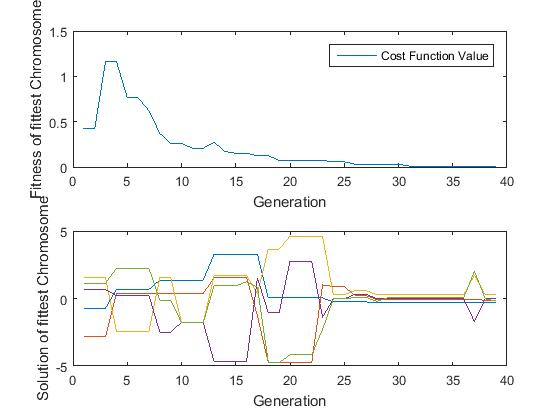
\includegraphics[width=0.5\linewidth]{ga_tf1_s1_c1a}}
\centerline{Trial 1}
\centerline{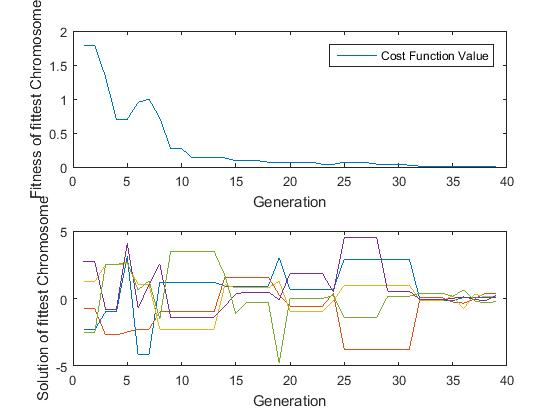
\includegraphics[width=0.5\linewidth]{ga_tf1_s1_c1b}}
\centerline{Trial 2}
\centerline{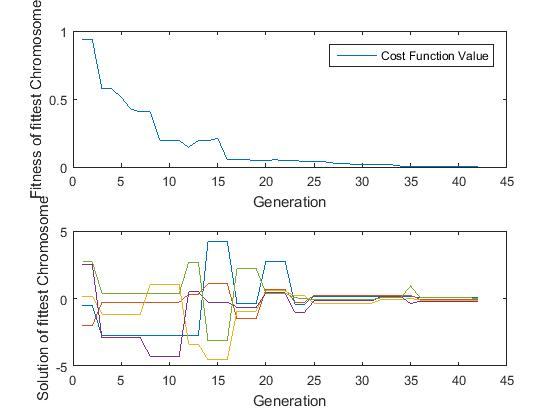
\includegraphics[width=0.5\linewidth]{ga_tf1_s1_c1c}}
\centerline{Trial 3}

\textbf{Genetic Algorithm} The GA results below used the \textit{Tournament Selection} and a \textit{Triple-Point Crossover}\\
\centerline{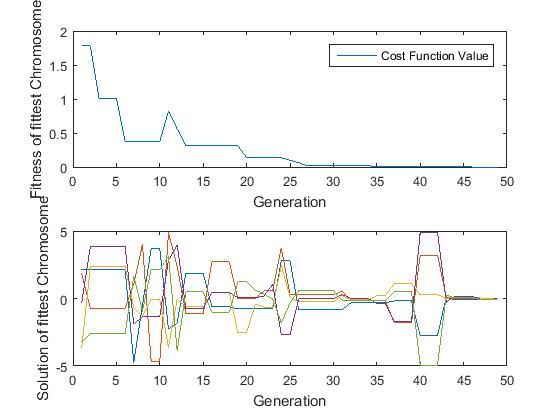
\includegraphics[width=0.5\linewidth]{ga_tf1_s1_c2a}}
\centerline{Trial 1}
\centerline{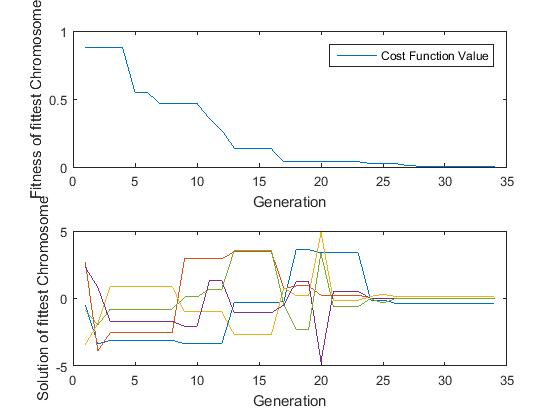
\includegraphics[width=0.5\linewidth]{ga_tf1_s1_c2b}}
\centerline{Trial 2}
\centerline{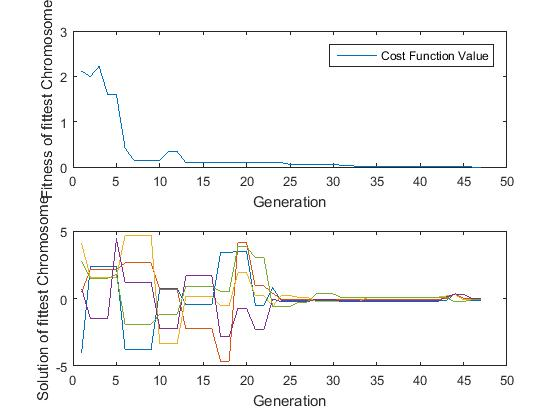
\includegraphics[width=0.5\linewidth]{ga_tf1_s1_c2c}}
\centerline{Trial 3}

\textbf{Simulated Annealing} The SA results are shown below:\\
\centerline{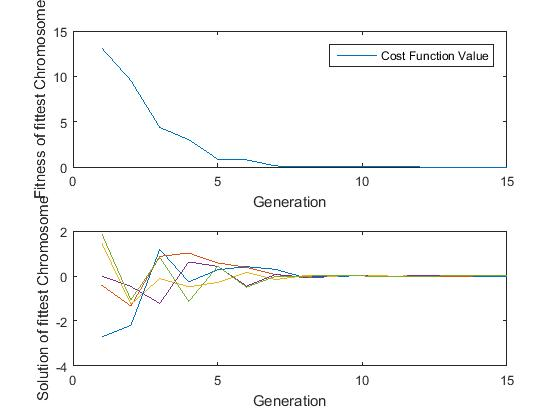
\includegraphics[width=0.5\linewidth]{sa_tf1_a}}
\centerline{Trial 1}
\centerline{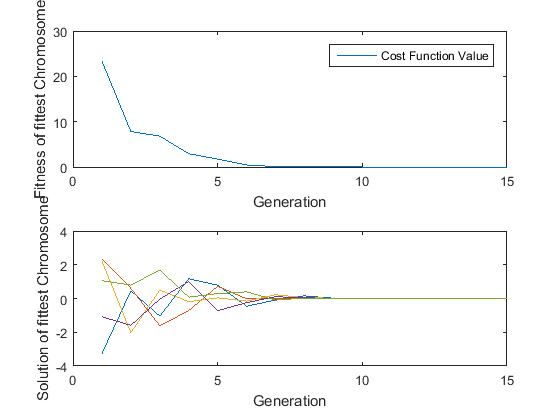
\includegraphics[width=0.5\linewidth]{sa_tf1_b}}
\centerline{Trial 2}
\centerline{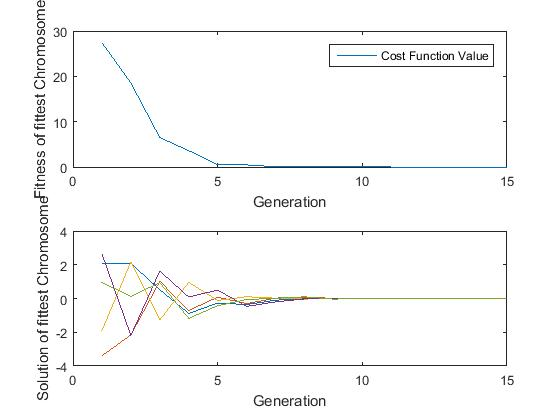
\includegraphics[width=0.5\linewidth]{sa_tf1_c}}
\centerline{Trial 3}

\textbf{Hybrid Simulated Annealing} The SAGA results are shown below:\\
\centerline{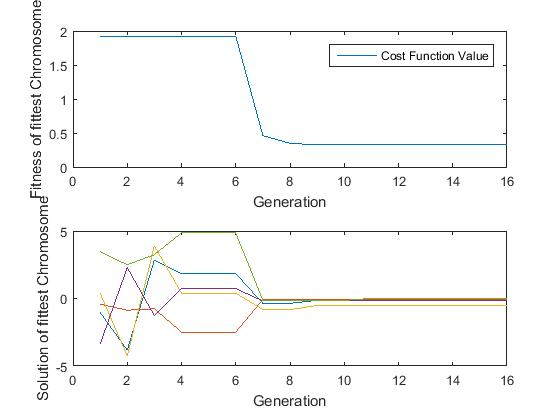
\includegraphics[width=0.5\linewidth]{saga_tf1_a}}
\centerline{Trial 1}
\centerline{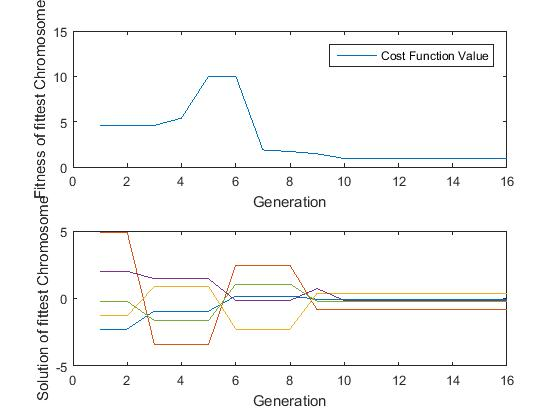
\includegraphics[width=0.5\linewidth]{saga_tf1_b}}
\centerline{Trial 2}
\centerline{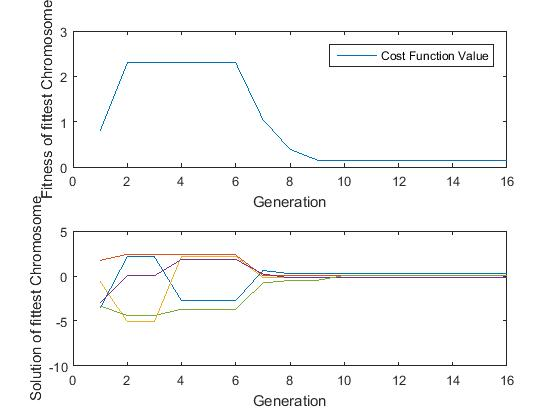
\includegraphics[width=0.5\linewidth]{saga_tf1_c}}
\centerline{Trial 3}

\textbf{On Accuracy and Runtime in De Jong's Function}\\
GA - Tournament Selection - Single Point Crossover Average Final Fitness: 8.7131e-08\\
GA - Tournament Selection - Triple Point Crossover Average Final Fitness: 1.0391e-07\\
Simulated Annealing Average Final Fitness: 2.4043e-05\\
SAGA - Boltzman Trial Average Final Fitness: 0.4725\\

GA - Tournament Selection - Single Point Crossover Average Time: 5.0003s\\
GA - Tournament Selection - Triple Point Crossover Average Time: 5.7281s\\
Simulated Annealing Average Time: 8.0448s\\
SAGA - Boltzman Trial Average Time: 33.1052s\\

\subsection{Axis Parallel Hyper-Ellipsoid Function}
\textbf{Genetic Algorithm} The GA results below used the \textit{Tournament Selection} and a \textit{Single-Point Crossover}\\
\centerline{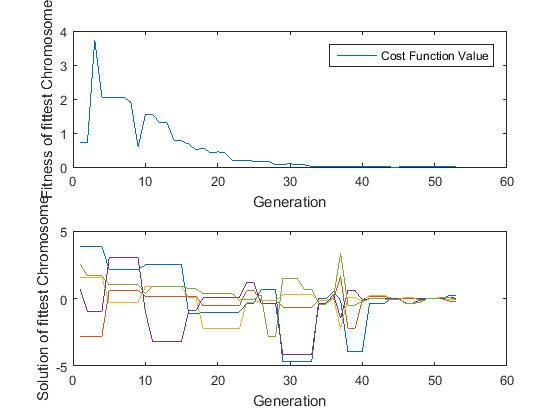
\includegraphics[width=0.5\linewidth]{ga_tf2_s1_c1a}}
\centerline{Trial 1}
\centerline{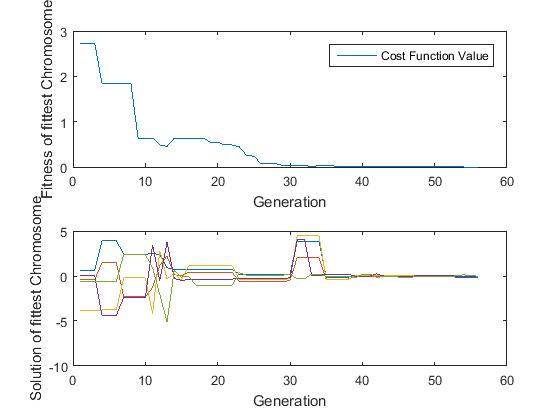
\includegraphics[width=0.5\linewidth]{ga_tf2_s1_c1b}}
\centerline{Trial 2}
\centerline{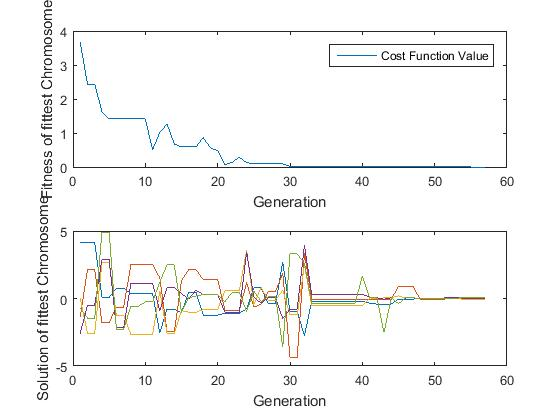
\includegraphics[width=0.5\linewidth]{ga_tf2_s1_c1c}}
\centerline{Trial 3}

\textbf{Genetic Algorithm} The GA results below used the \textit{Tournament Selection} and a \textit{Triple-Point Crossover}\\
\centerline{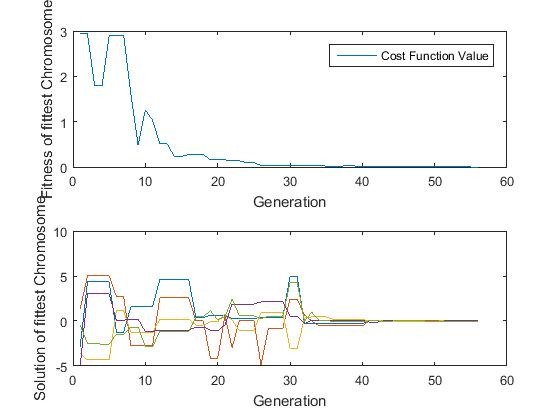
\includegraphics[width=0.5\linewidth]{ga_tf2_s1_c2a}}
\centerline{Trial 1}
\centerline{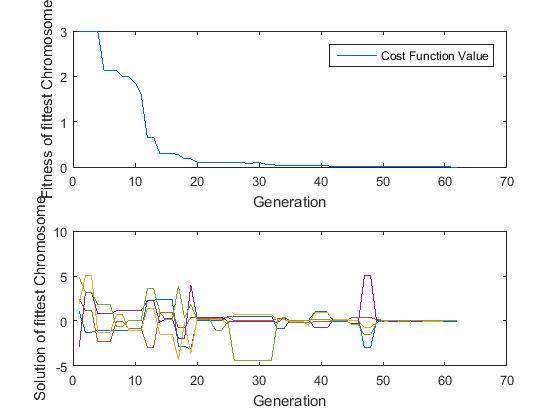
\includegraphics[width=0.5\linewidth]{ga_tf2_s1_c2b}}
\centerline{Trial 2}
\centerline{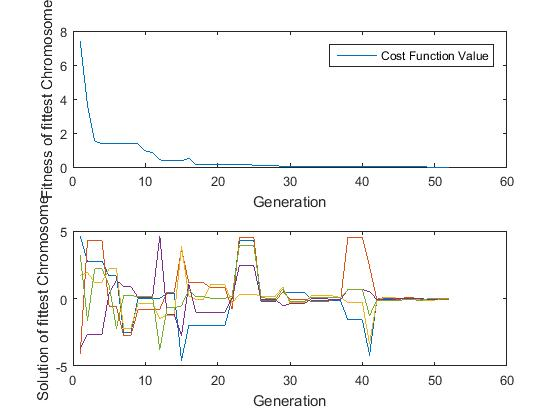
\includegraphics[width=0.5\linewidth]{ga_tf2_s1_c2c}}
\centerline{Trial 3}

\textbf{Simulated Annealing} The SA results are shown below:\\
\centerline{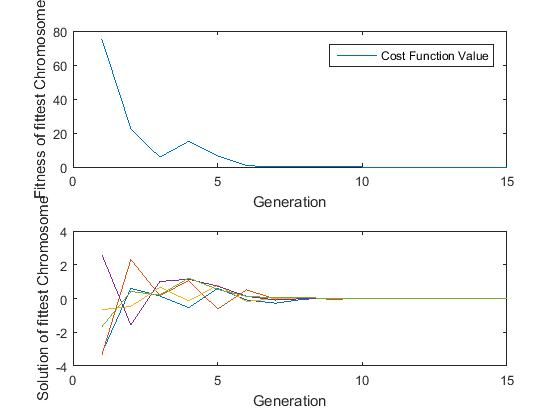
\includegraphics[width=0.5\linewidth]{sa_tf2_a}}
\centerline{Trial 1}
\centerline{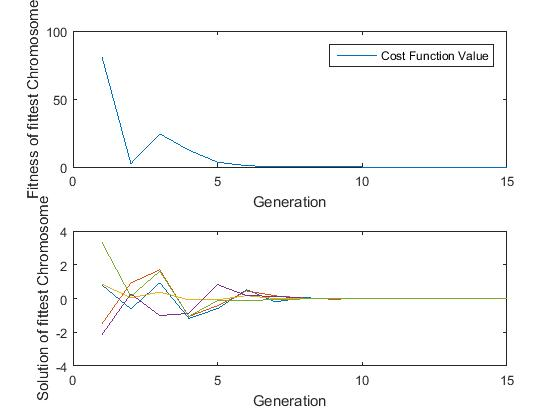
\includegraphics[width=0.5\linewidth]{sa_tf2_b}}
\centerline{Trial 2}
\centerline{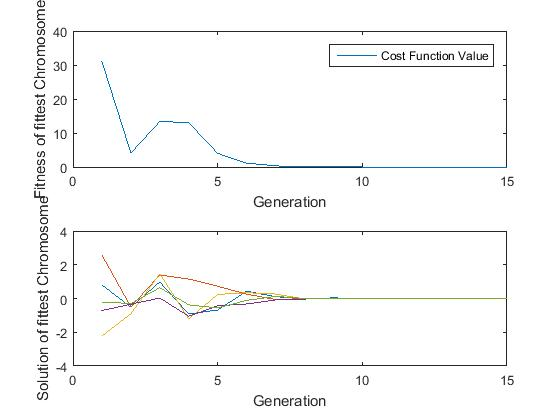
\includegraphics[width=0.5\linewidth]{sa_tf2_c}}
\centerline{Trial 3}

\textbf{Hybrid Simulated Annealing} The SAGA results are shown below:\\
\centerline{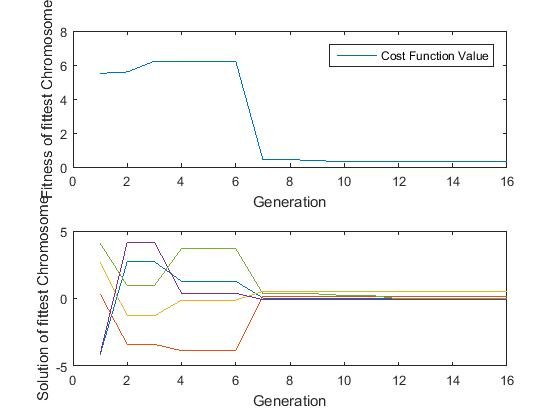
\includegraphics[width=0.5\linewidth]{saga_tf2_a}}
\centerline{Trial 1}
\centerline{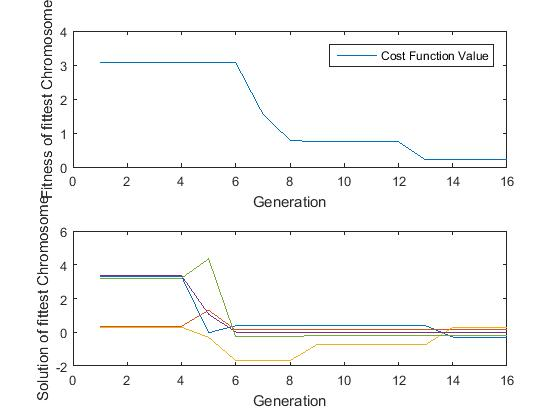
\includegraphics[width=0.5\linewidth]{saga_tf2_b}}
\centerline{Trial 2}
\centerline{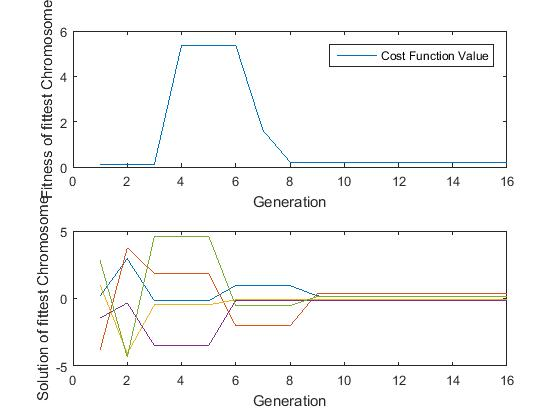
\includegraphics[width=0.5\linewidth]{saga_tf2_c}}
\centerline{Trial 3}

\textbf{On Accuracy and Runtime in the Axis Parallel Hyper-Ellipsoid Function}\\
GA - Tournament Selection - Single Point Crossover Average Final Fitness: 7.5826e-07\\
GA - Tournament Selection - Triple Point Crossover Average Final Fitness: 4.5725e-08\\
Simulated Annealing Average Final Fitness: 8.8213e-05\\
SAGA - Boltzman Trial Average Final Fitness: 0.2415\\

GA - Tournament Selection - Single Point Crossover Average Time: 6.9705s\\
GA - Tournament Selection - Triple Point Crossover Average Time: 7.8155s\\
Simulated Annealing Average Time: 9.7563s\\
SAGA - Boltzman Trial Average Time: 39.6909s\\

\subsection{Rotated Hyper-Ellipsoid Function}
\textbf{Genetic Algorithm} The GA results below used the \textit{Tournament Selection} and a \textit{Single-Point Crossover}\\
\centerline{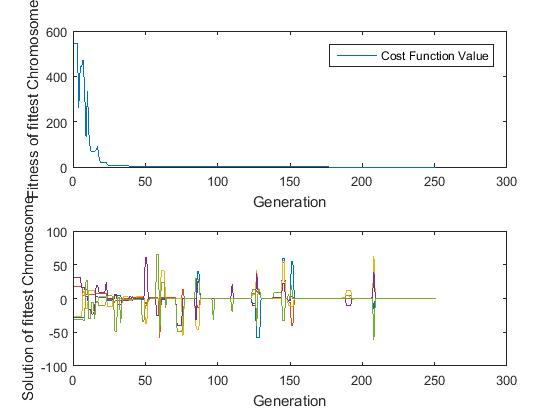
\includegraphics[width=0.5\linewidth]{ga_tf3_s1_c1a}}
\centerline{Trial 1}
\centerline{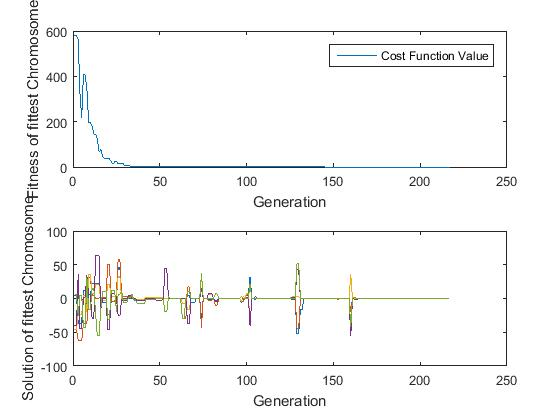
\includegraphics[width=0.5\linewidth]{ga_tf3_s1_c1b}}
\centerline{Trial 2}
\centerline{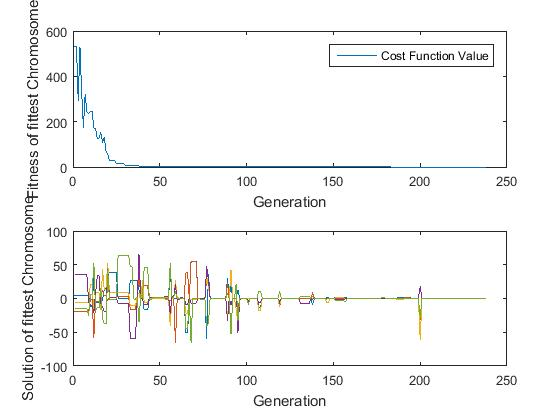
\includegraphics[width=0.5\linewidth]{ga_tf3_s1_c1c}}
\centerline{Trial 3}

\textbf{Genetic Algorithm} The GA results below used the \textit{Tournament Selection} and a \textit{Triple-Point Crossover}\\
\centerline{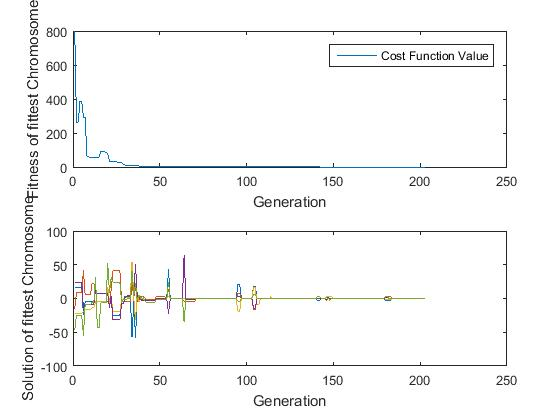
\includegraphics[width=0.5\linewidth]{ga_tf3_s1_c2a}}
\centerline{Trial 1}
\centerline{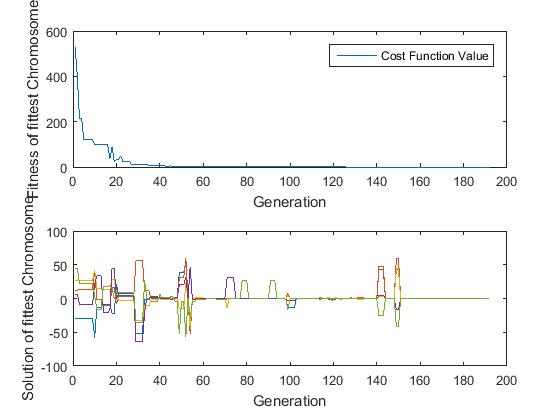
\includegraphics[width=0.5\linewidth]{ga_tf3_s1_c2b}}
\centerline{Trial 2}
\centerline{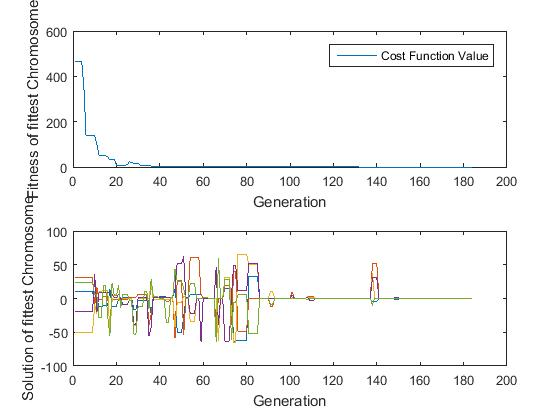
\includegraphics[width=0.5\linewidth]{ga_tf3_s1_c2c}}
\centerline{Trial 3}

\textbf{Simulated Annealing} The SA results are shown below:\\
\centerline{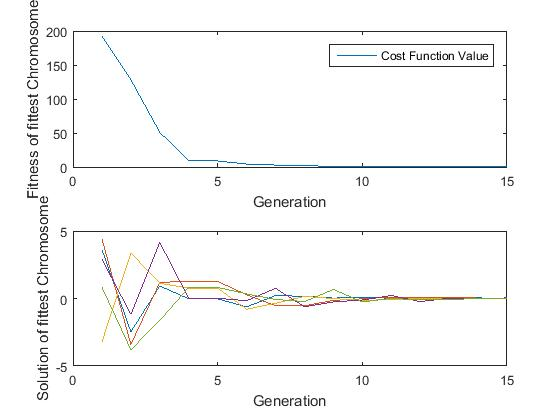
\includegraphics[width=0.5\linewidth]{sa_tf3_a}}
\centerline{Trial 1}
\centerline{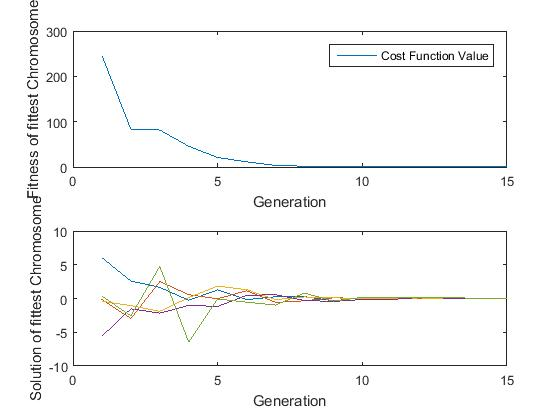
\includegraphics[width=0.5\linewidth]{sa_tf3_b}}
\centerline{Trial 2}
\centerline{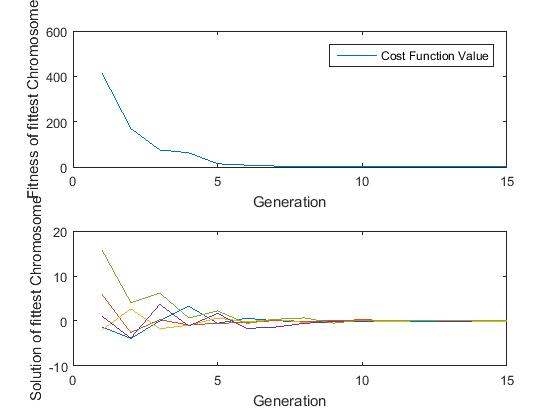
\includegraphics[width=0.5\linewidth]{sa_tf3_c}}
\centerline{Trial 3}

\textbf{Hybrid Simulated Annealing} The SAGA results are shown below:\\
\centerline{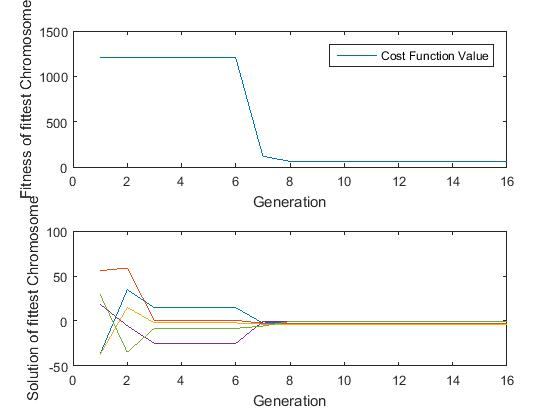
\includegraphics[width=0.5\linewidth]{saga_tf3_a}}
\centerline{Trial 1}
\centerline{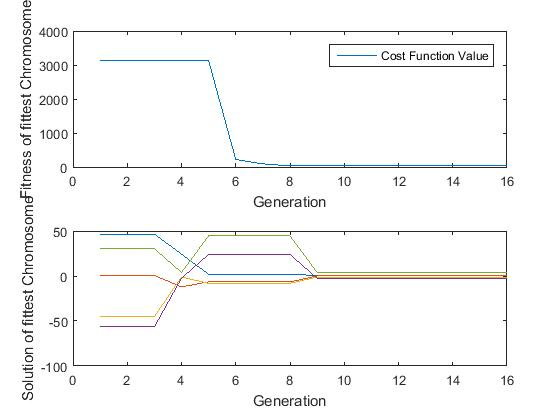
\includegraphics[width=0.5\linewidth]{saga_tf3_b}}
\centerline{Trial 2}
\centerline{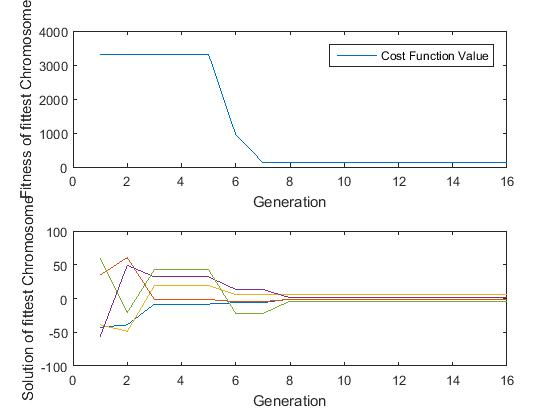
\includegraphics[width=0.5\linewidth]{saga_tf3_c}}
\centerline{Trial 3}

\textbf{On Accuracy and Runtime in the Rotated Hyper-Ellipsoid Function}\\
GA - Tournament Selection - Single Point Crossover Average Final Fitness: 9.2024e-07\\
GA - Tournament Selection - Triple Point Crossover Average Final Fitness: 1.0930e-06\\
Simulated Annealing Average Final Fitness: 0.0091\\
SAGA - Boltzman Trial Average Final Fitness: 75.7499\\

GA - Tournament Selection - Single Point Crossover Average Time: 33.9621s\\
GA - Tournament Selection - Triple Point Crossover Average Time: 32.7585s\\
Simulated Annealing Average Time: 10.4437s\\
SAGA - Boltzman Trial Average Time: 38.6104s\\

\subsection{Rastrigin's Function}
\textbf{Genetic Algorithm} The GA results below used the \textit{Tournament Selection} and a \textit{Single-Point Crossover}\\
\centerline{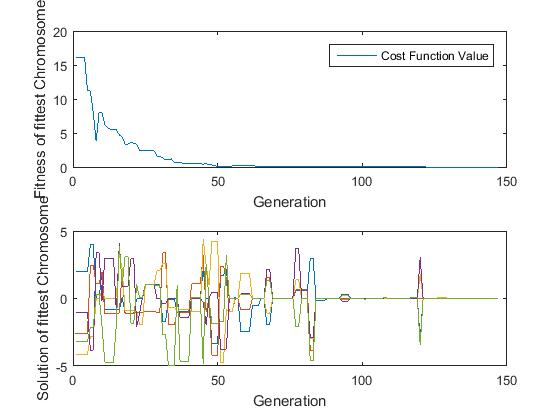
\includegraphics[width=0.5\linewidth]{ga_tf4_s1_c1a}}
\centerline{Trial 1}
\centerline{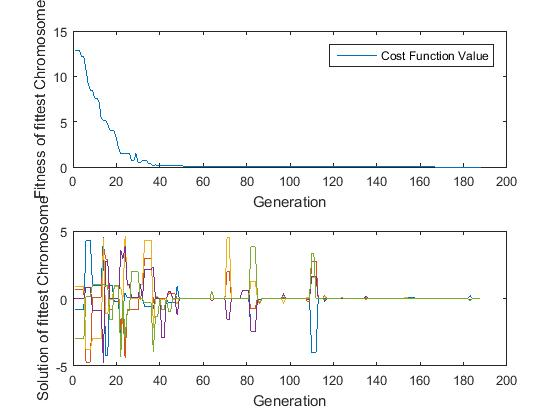
\includegraphics[width=0.5\linewidth]{ga_tf4_s1_c1b}}
\centerline{Trial 2}
\centerline{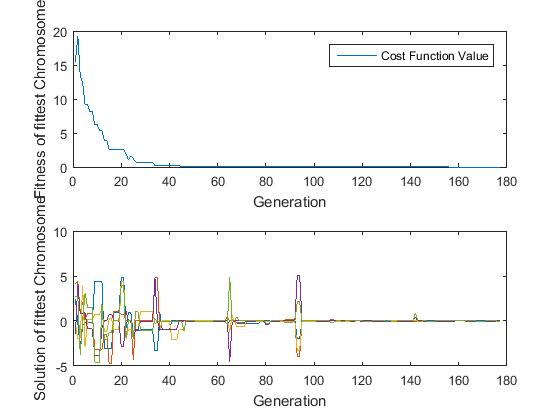
\includegraphics[width=0.5\linewidth]{ga_tf4_s1_c1c}}
\centerline{Trial 3}

\textbf{Genetic Algorithm} The GA results below used the \textit{Tournament Selection} and a \textit{Triple-Point Crossover}\\
\centerline{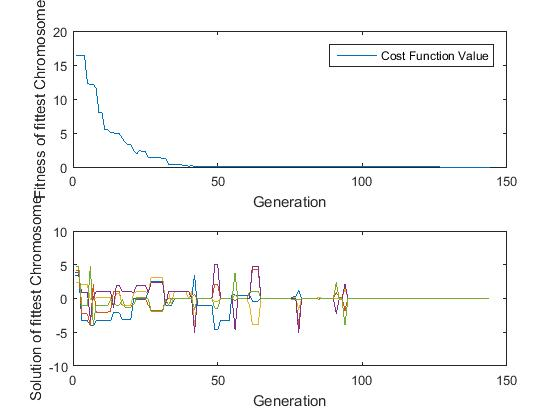
\includegraphics[width=0.5\linewidth]{ga_tf4_s1_c2a}}
\centerline{Trial 1}
\centerline{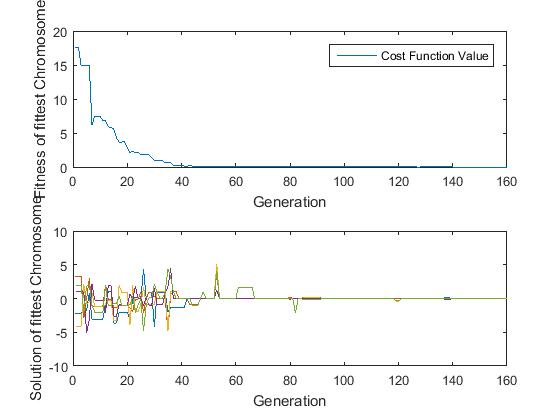
\includegraphics[width=0.5\linewidth]{ga_tf4_s1_c2b}}
\centerline{Trial 2}
\centerline{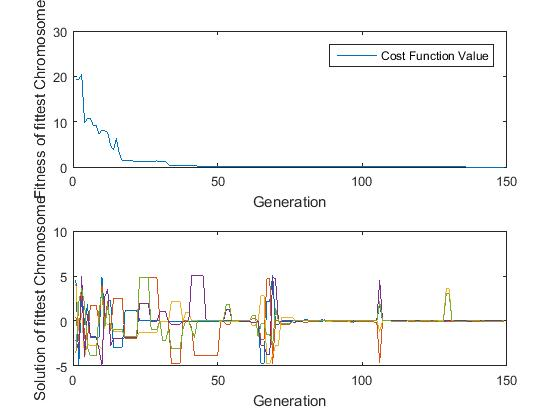
\includegraphics[width=0.5\linewidth]{ga_tf4_s1_c2c}}
\centerline{Trial 3}

\textbf{Simulated Annealing} The SA results are shown below:\\
\centerline{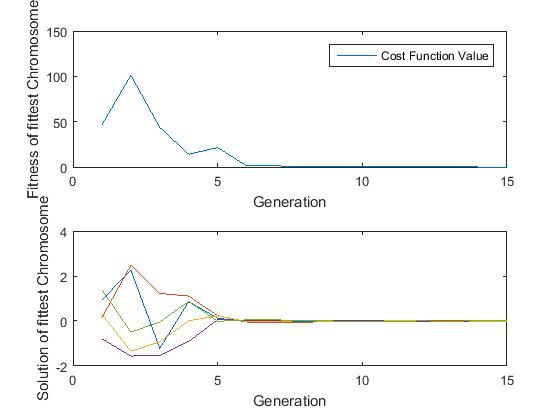
\includegraphics[width=0.5\linewidth]{sa_tf4_a}}
\centerline{Trial 1}
\centerline{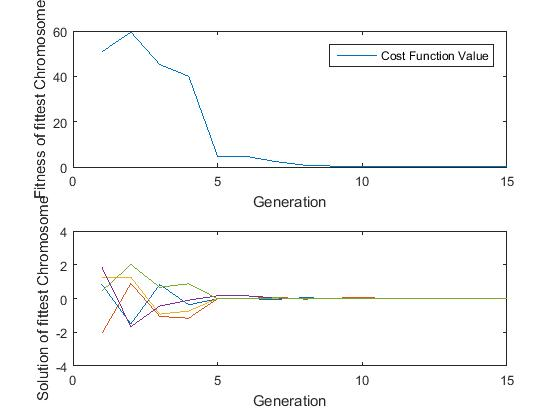
\includegraphics[width=0.5\linewidth]{sa_tf4_b}}
\centerline{Trial 2}
\centerline{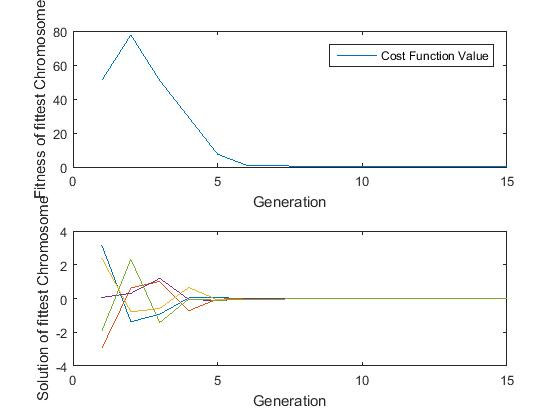
\includegraphics[width=0.5\linewidth]{sa_tf4_c}}
\centerline{Trial 3}

\textbf{Hybrid Simulated Annealing} The SAGA results are shown below:\\
\centerline{\includegraphics[width=0.5\linewidth]{saga_tf4_a}}
\centerline{Trial 1}
\centerline{\includegraphics[width=0.5\linewidth]{saga_tf4_b}}
\centerline{Trial 2}
\centerline{\includegraphics[width=0.5\linewidth]{saga_tf4_c}}
\centerline{Trial 3}

\textbf{On Accuracy and Runtime in Rasrigin's Function}\\
GA - Tournament Selection - Single Point Crossover Average Final Fitness: 4.6318e-07\\
GA - Tournament Selection - Triple Point Crossover Average Final Fitness: 5.4631e-07\\
Simulated Annealing Average Final Fitness: 0.0041\\
SAGA - Boltzman Trial Average Final Fitness: 10.1396\\

GA - Tournament Selection - Single Point Crossover Average Time: 28.2559s\\
GA - Tournament Selection - Triple Point Crossover Average Time: 25.9490s\\
Simulated Annealing Average Time: 11.7933s\\
SAGA - Boltzman Trial Average Time: 42.7257s\\

\subsection{Ackley's Function}
\textbf{Genetic Algorithm} The GA results below used the \textit{Tournament Selection} and a \textit{Single-Point Crossover}\\
\centerline{\includegraphics[width=0.5\linewidth]{ga_tf5_s1_c1a}}
\centerline{Trial 1}
\centerline{\includegraphics[width=0.5\linewidth]{ga_tf5_s1_c1b}}
\centerline{Trial 2}
\centerline{\includegraphics[width=0.5\linewidth]{ga_tf5_s1_c1c}}
\centerline{Trial 3}

\textbf{Genetic Algorithm} The GA results below used the \textit{Tournament Selection} and a \textit{Triple-Point Crossover}\\
\centerline{\includegraphics[width=0.5\linewidth]{ga_tf5_s1_c2a}}
\centerline{Trial 1}
\centerline{\includegraphics[width=0.5\linewidth]{ga_tf5_s1_c2b}}
\centerline{Trial 2}
\centerline{\includegraphics[width=0.5\linewidth]{ga_tf5_s1_c2c}}
\centerline{Trial 3}

\textbf{Simulated Annealing} The SA results are shown below:\\
\centerline{\includegraphics[width=0.5\linewidth]{sa_tf5_a}}
\centerline{Trial 1}
\centerline{\includegraphics[width=0.5\linewidth]{sa_tf5_b}}
\centerline{Trial 2}
\centerline{\includegraphics[width=0.5\linewidth]{sa_tf5_c}}
\centerline{Trial 3}

\textbf{Hybrid Simulated Annealing} The SAGA results are shown below:\\
\centerline{\includegraphics[width=0.5\linewidth]{saga_tf5_a}}
\centerline{Trial 1}
\centerline{\includegraphics[width=0.5\linewidth]{saga_tf5_b}}
\centerline{Trial 2}
\centerline{\includegraphics[width=0.5\linewidth]{saga_tf5_c}}
\centerline{Trial 3}

\textbf{On Accuracy and Runtime in Ackley's Function}\\
GA - Tournament Selection - Single Point Crossover Average Final Fitness: 1.8221e-06\\
GA - Tournament Selection - Triple Point Crossover Average Final Fitness: 2.3472e-06\\
Simulated Annealing Average Final Fitness: 0.0669\\
SAGA - Boltzman Trial Average Final Fitness: 6.3355\\

GA - Tournament Selection - Single Point Crossover Average Time: 134.6147s\\
GA - Tournament Selection - Triple Point Crossover Average Time: 99.7033s\\
Simulated Annealing Average Time:  9.7725s\\
SAGA - Boltzman Trial Average Time: 36.6362s\\

\section{Conclusion}
After a series of tests, trials and runs. The results were gathered as mentioned above. To indeed be able to draw an interpretation or observation of the behaviour and performance of each algorithm, a much more numerous trials has to be made. But with that said, the following observations seen on the behaviour and performance of each algorithm on each problem are discussed in the following. On the much more obvious observation, the Genetic Algorithm and the Simulated Annealing are accurate in solving or looking for the global minimum (solution). Meanwhile, the Hybrid Simulated Annealing never came close as the fitness function or cost function are significantly not close to zero as this is a minimization problem. Also, both the GA and SA have obtained the solution in a considerably fast time as opposed to the SAGA. So with this, it can be inferred that the GA and SA are much more better the SAGA (as how each of them is implemented in the program). But to differentiate the GA and SA, a difference in their behaviour in looking for the solution is very much observable in the graphs shown above. The GA takes a much more random walk or random guesses due to mutations as observed from their frequent fluctuations in looking for the solution. The movement of the GA is rather sharp and crispy as opposed to that of the behaviour of the SA. The SA, as observed from the graphs, draws a much more smoother flow of looking for the solution. This is due to the continuous cooling of the system that restricts the program from making sharp and crispy fluctuations. With all of that said, it is safe therefore to say that both the Genetic Algorithm and the Simulated Annealing, though have different behaviours, are much more capable in looking and finding for the solution as opposed to the Hybrid Simulated Annealing.

\section{References}
[1] Molga, M. and Smutnicki, C., "Test Functions for Optimization Needs", 2005
\\

[2] Hermawanto, D., "Genetic Algorithm for Solving Simple Mathematical Equality Problem", Indonesian Institute of Sciences, n.d.
\\

[3] de Weck O.,  "Simulated Annealing: A Basic Introduction", Massachusetts Institute of Technology, 2010 
\end{document}
